\documentclass[.../Dokumentation.tex]{subfiles}
\begin{document}
\subsection{Fahrzeuge}\label{sec-ita2-cars}
Um die in \ref{sec-ita1-result} identifizierten Probleme hinsichtlich des 
Platzbedarfs zu lösen, wurden die Maße des Fahrzeugs angepasst.
Da der erste Eindruck der Beschaffenheit des in Abbildung 
\ref{fig-car-firstPrint} gezeigten Drucks hinsichtlich seiner Stabilität 
die anfänglichen Erwartungen übertroffen hat, wurden zunächst die zu den Seiten 
des Fahrzeugs gelegenen Außenwände der Aussparung in ihrer Stärke halbiert.
Weiter wurde das gesamte Modell in der Länge erweitert und der Hohlraum im 
Fahrzeug so weit wie möglich in diese Richtung vergrößert. Hierdurch soll 
zukünftigen Platz-Engpässen vorgebeugt werden.\\
An dieser Stelle wurde ein weiterer Druck durchgeführt, um das 
Zusammenspiel mit Rädern und Befestigung zu prüfen. Hierbei wurden alle 
Einzelteile für den Druck in einem einzigen Drucker arrangiert.
\begin{figure}[H]
\begin{center}
    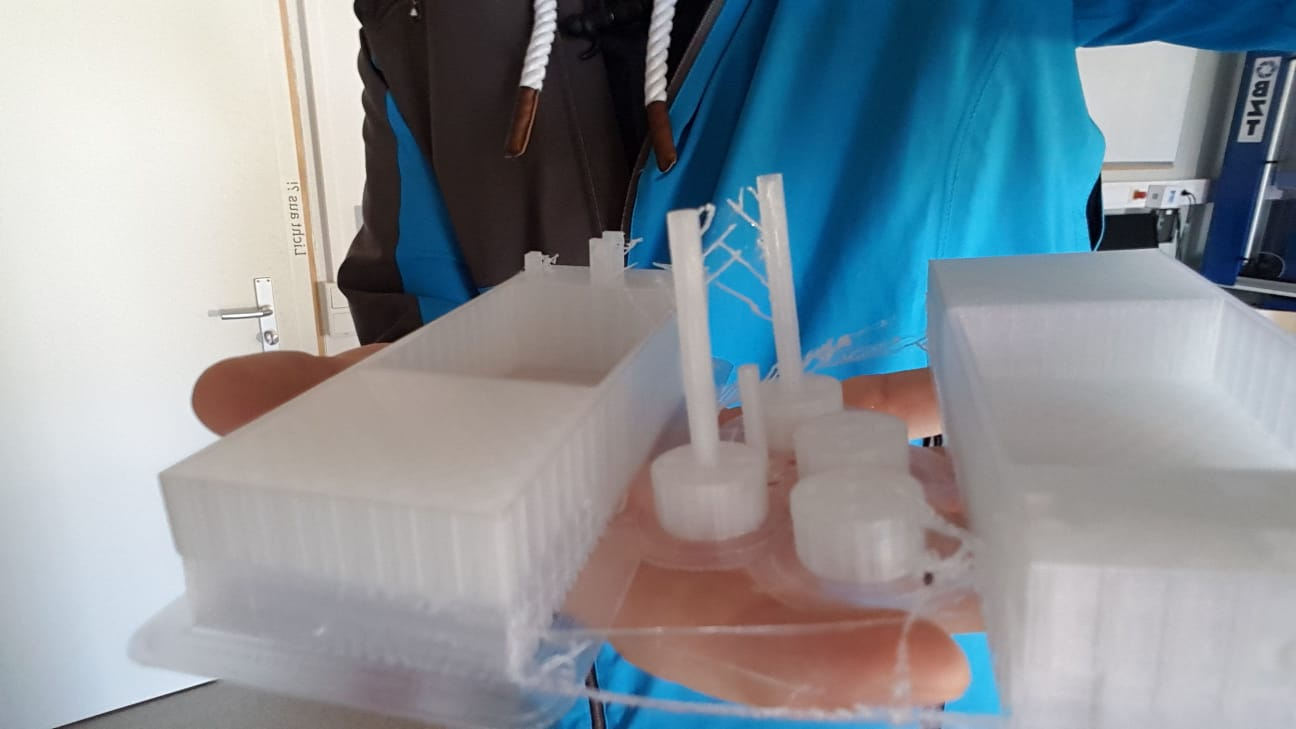
\includegraphics[
        width=0.5\linewidth,
    ]{imgs/car_2ndPrint.jpeg}
    \caption{Alle Komponenten eines Fahrzeugs aus einem Druck}
    \label{fig-car-2ndPrint}
\end{center}
\end{figure}
\begin{figure}[H]
\begin{center}
    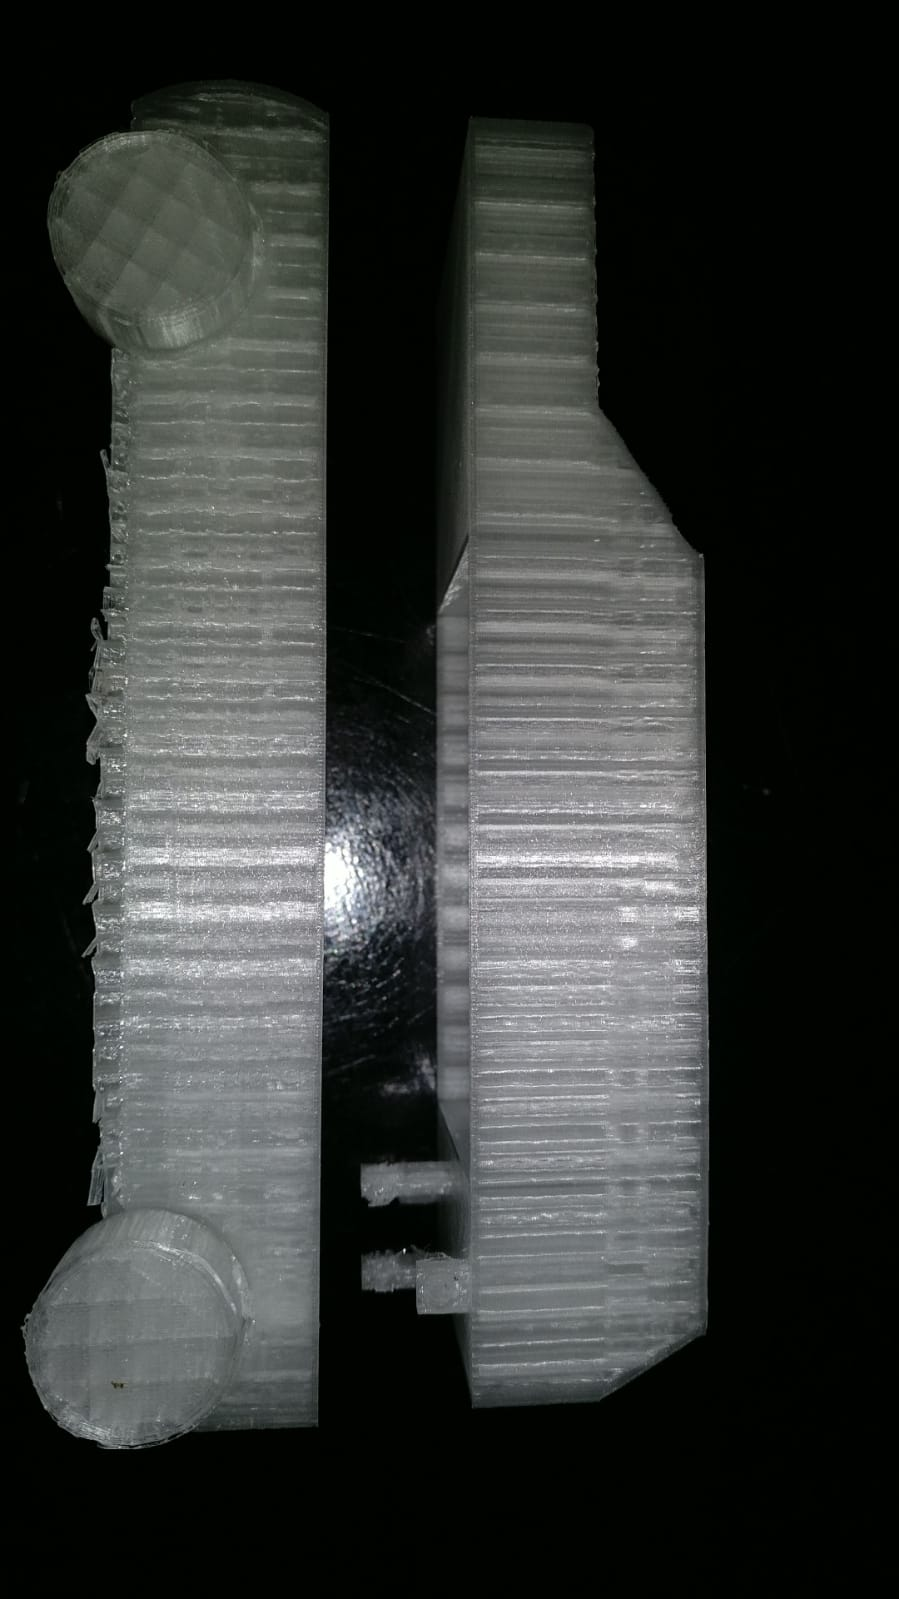
\includegraphics[
        width=0.5\linewidth,
        angle=90,
        origin=c,
    ]{imgs/car_2ndPrint_assembled.jpeg}
    \vspace*{-2.75cm}
    \caption{Fahrzeughälften mit montierten Rädern}
    \label{fig-car-2ndPrint-assembled}
\end{center}
\end{figure}
\noindent
Während Abbildung \ref{fig-car-2ndPrint} das Ergebnis dieses Drucks zeigt, 
vermittelt Abbildung \ref{fig-car-2ndPrint-assembled} einen Eindruck 
von Form und Dimensionen des fertigen Produkts.
\end{document}